%!TEX root = ../../super_main.tex
\part{Third Sprint}
\label{par:third_sprint}

\chapter{Sprint Overview}
In the third sprint, our group handed over the task of creating and maintaining the shared GUI components of the project (commonly referred to as \gc) to another group. This transfer of responsibility has been done in order for our group to finish the \ct before the start of the fourth sprint. The workload of both the \ct and the \gc was too much for our group to guarantee that we could complete both tasks. The focus of this sprint is therefore to finish up the \ct and ensure that it is stable after this sprint.\\

At the start of the third sprint, the application was in a state where guardians were able to create categories and view their content. It was not possible to add pictograms to a category without hardcoding them. It was possible to change user to a citizen profile and view which categories have already been made on a child profile and watch their content. \\

What is currently missing is the feature that opens \ps and allows a user to search for specific pictograms and adding them to a desired category. Furthermore, the concept of transferring guardian/institution categories onto citizen profiles and being able to modify individual citizen categories without affecting any of the others. Another missing feature is the possibility of editing a guardian/institution category and then cascading any changes down onto every citizen category which is a child of this super-category. In addition, some memory issues have been discovered when a list of pictograms in a category becomes too large which has to be solved. 

%!TEX root = ../../../super_main.tex

\chapter{Issues and Solutions}

\todo{Write about our design meeting?}

%!TEX root = ../../../super_main.tex

\section{Using Pictosearch}
\label{sec:using_pictosearch}

When using the \ct, a common use case is that the user wants to find and use pictograms in various situations, for instance as an icon for a category or populating categories. For this sake, we utilize an application developed for the \giraf software suite called \ps. This application includes an \androidinline{Activity} subclass called \androidinline{PictoAdminMain} which is able to return one or more pictograms to the calling \androidinline{Activity} when a user enters a search string and selects pictograms. 
\\\\
\ps is used in three ways in the \ct: When creating a category, when editing a category, and when populating the category with pictograms. In order to use a remote \androidinline{Activity} from another application for this kind of request we utilize the \androidinline{Intent}-class. An \androidinline{Activity} is, using an \androidinline{Intent}-class instance, able to make a request to another activity asking for some result cross the operating system, in our case a very specific request to \ps asking for IDs of pictograms. 

\lstinputlisting[
    style = Java,
    caption = {A request for a single pictogram.},
    label = {lst:intent_example},
]{content/sprint_3/issues_solutions/intent_example.java}

The code in \lstref{lst:intent_example} shows an example of how we, using an \androidinline{Intent} instance, open \ps and ask for a single pictogram. The thing to notice is that we are able to ask \ps for a single pictogram using the \androidinline{PICTO_SEARCH_SINGLE_TAG}, where the user is only able to select a single pictogram. This is used when picking an icon for category, whereas \androidinline{PICTO_SEARCH_MULTI_TAG} is used when populating a category. 
\\\\
When a user has selected the desired pictogram(s), he is returned to the \ct, where an event is raised causing the method \androidinline{onActivityResult} to be called. Using the request code (\androidinline{GET_SINGLE_PICTOGRAM} in \lstref{lst:intent_example}), this method knows what request has been answered and can now perform some action based on this, which in this case is to store the identifier for the pictogram in the category it was picked for.



%!TEX root = ../../../super_main.tex

\section{ShowcaseView}
\label{sec:showcaseview}

It was our initial intention, as described in \secref{sec:home_screen} and seen in \figref{fig:improved_design_category_selected_1}, \figref{fig:improved_design_category_selected_2}, to have some arrows with accompanying text to help guide the users with their first use of the application. We were however unable to find a library which implemented such an arrow overlay. We did however find another library called \androidinline{ShowcaseView}. 

\androidinline{ShowcaseView} is the name of a class and a library licensed under the Apache License, Version 2.0, originally created by Alex Curran and hosted on GitHub \parencite{showcaseview_by_alex_curran}. %https://github.com/amlcurran/ShowcaseView

The idea is then that we want to be able to guide the users, by showcasing areas of the application, through the first visit of the application and later on demand by clicking a help button. 

\androidinline{ShowcaseView} is a subclass of \androidinline{View} which, in combination with the rest of the library, can be used to showcase one or more areas of the screen. An area is showcased by putting a dark transparent overlay over the screen and then letting the showcased area, in a circle, be completely transparent along with some text as seen in \figref{fig:showcaseview_example}.

\begin{figure}[!htbp]
    \centering
    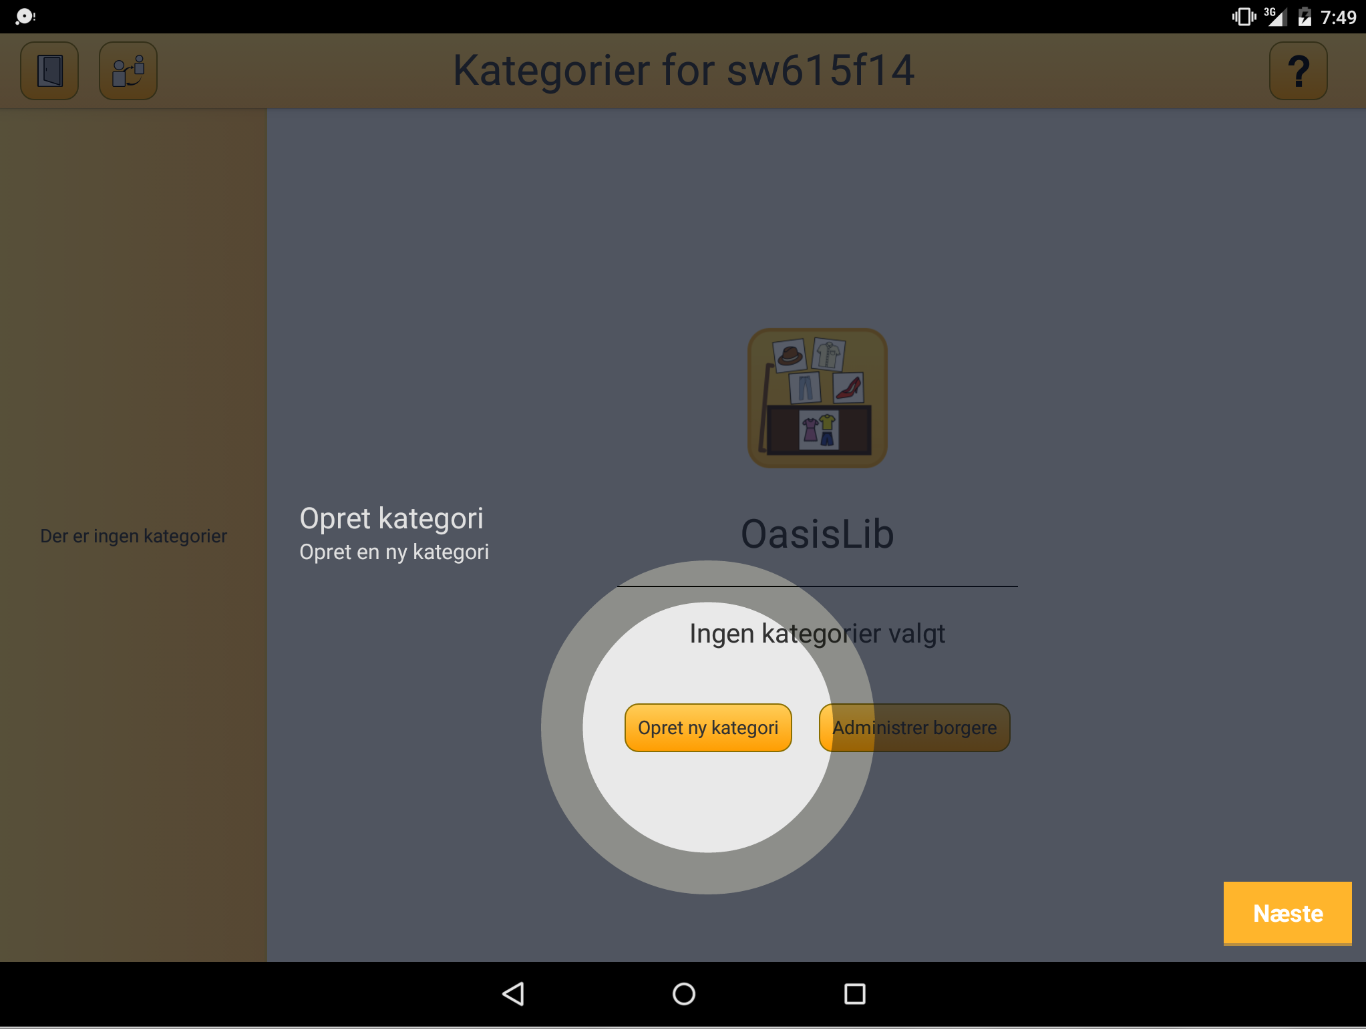
\includegraphics[width=0.75\textwidth]{sprint_three/showcaseview_example}
    \caption{Example of the \androidinline{ShowcaseView}}
    \label{fig:showcaseview_example}
\end{figure}

\subsection{Apache license}
As mentioned, this library is licensed under the Apache License 2.0 which allows for modifications and redistribution as long as certain requirements are met \parencite{apache2license}. In summary: The original copyright holder has to be credited, a full copy of the license must be distributed with the software, and changes must be stated.

\subsection{Additions to library}

% NOTICE !!!!!! ------------> Changes here should also be made in the NOTICE file <------------
The interface \androidinline{Target} has been changed to an abstract class. And subclasses of \androidinline{Target}, i.e. classes that previously implemented the interface \androidinline{Target}, has been modified with additional constructors, methods and properties to allow them to store their radius and a \androidinline{scaleMultiplier} (This was previously hard coded). The \androidinline{ViewTarget} subclass, of \androidinline{Target}, has been further modified to calculate its own radius based on its target view.  

The \androidinline{ShowcaseView} class and supporting classes have been modified to allow manual positioning of the help text for the ShowcaseView.\\ 
The \androidinline{TextDrawer} class has been modified to fix a problem with negative widths of the drawing area.
The additions to the library code is also described in a ``NOTICE'' file which is distributed with the code in the library's root directory. 

\subsection{Supporting code}

A new class \androidinline{ShowcaseManager} was introduced to help the transitions between different showcases. The class internally maintains a queue of objects implementing a \androidinline{Showcase} interface. A \androidinline{ShowcaseManager} instance will, when started with a call to its method \androidinline{start}, fetch the first \androidinline{Showcase} from its queue and call its \androidinline{configShowCaseView} method. This \androidinline{configShowCaseView} method is then supposed to configure the \androidinline{ShowcaseView} to match the first showcase by setting a subclass of \androidinline{Target} and more. The \androidinline{ShowcaseView} includes a next button which will, when clicked, invoke the next step by further emptying the queue and configure the next showcase.






%!TEX root = ../../../super_main.tex

\section{Locked Features for Citizens}
\label{sec:locked_features_for_citizens}

When viewing categories that have been assigned to a citizen profile it is not possible to change pictograms or names of categories, or copy their categories to other citizens, since the categories that are assigned to the citizen are child-categories of one that is located on the institution. This is enforced such that it is possible to propagate changes from the super-category to the child-categories, which for example could be changing the name of a category across all users that have the category. When locking features for citizens it has been decided that we use the \androidinline{View.setEnabled()} method on \androidinline{GirafButtons} with the value \androidinline{false}, which will automatically gray out the button. We then set a special click-listener on the button that is only active while the button is not enabled. This allows users of the \ct to press buttons that are disabled and then give us the possibility of telling the user the correct way of using the button. This has been implemented on two \androidinline{GirafButtons} in the \ct, namely the Settings- and the CopyCategory-Buttons, since these are not available to citizen categories. 

\begin{figure}[!htbp]
        \centering
        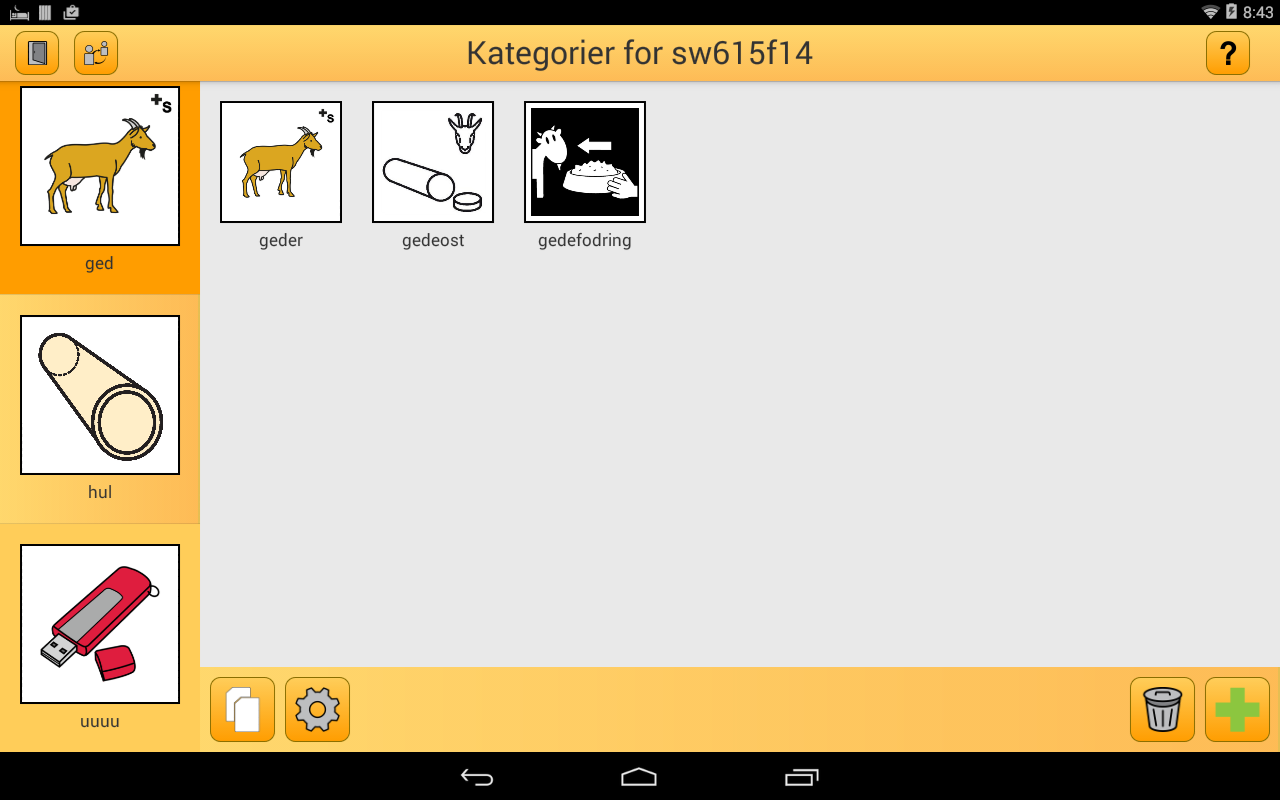
\includegraphics[width=0.75\textwidth]{sprint_three/locked_features_for_citizens/buttons_for_institution}
        \caption{\ct enabled buttons}
        \label{fig:ct_enabled_buttons}
\end{figure}

\begin{figure}[!htbp]
        \centering
        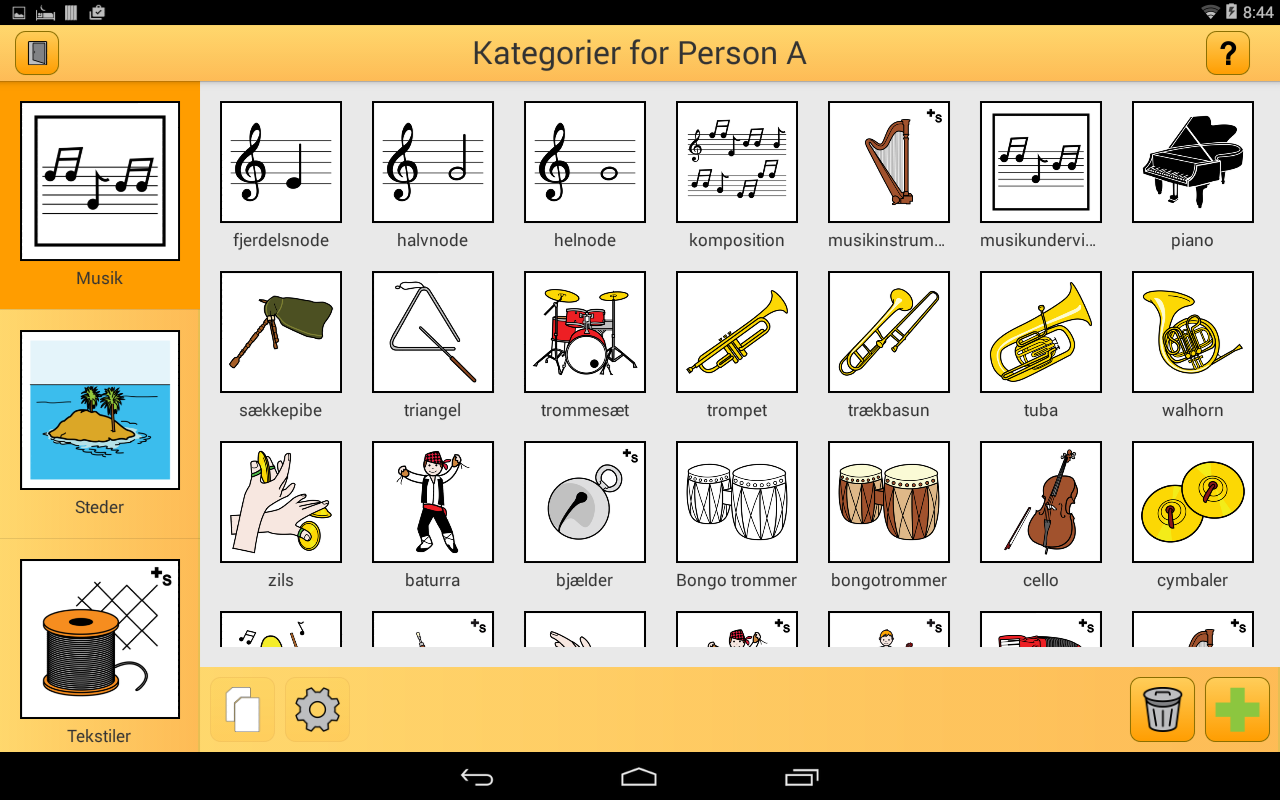
\includegraphics[width=0.75\textwidth]{sprint_three/locked_features_for_citizens/buttons_for_citizen}
        \caption{\ct disabled buttons}
        \label{fig:ct_disabled_buttons}
\end{figure}

\begin{figure}[!htbp]
        \centering
        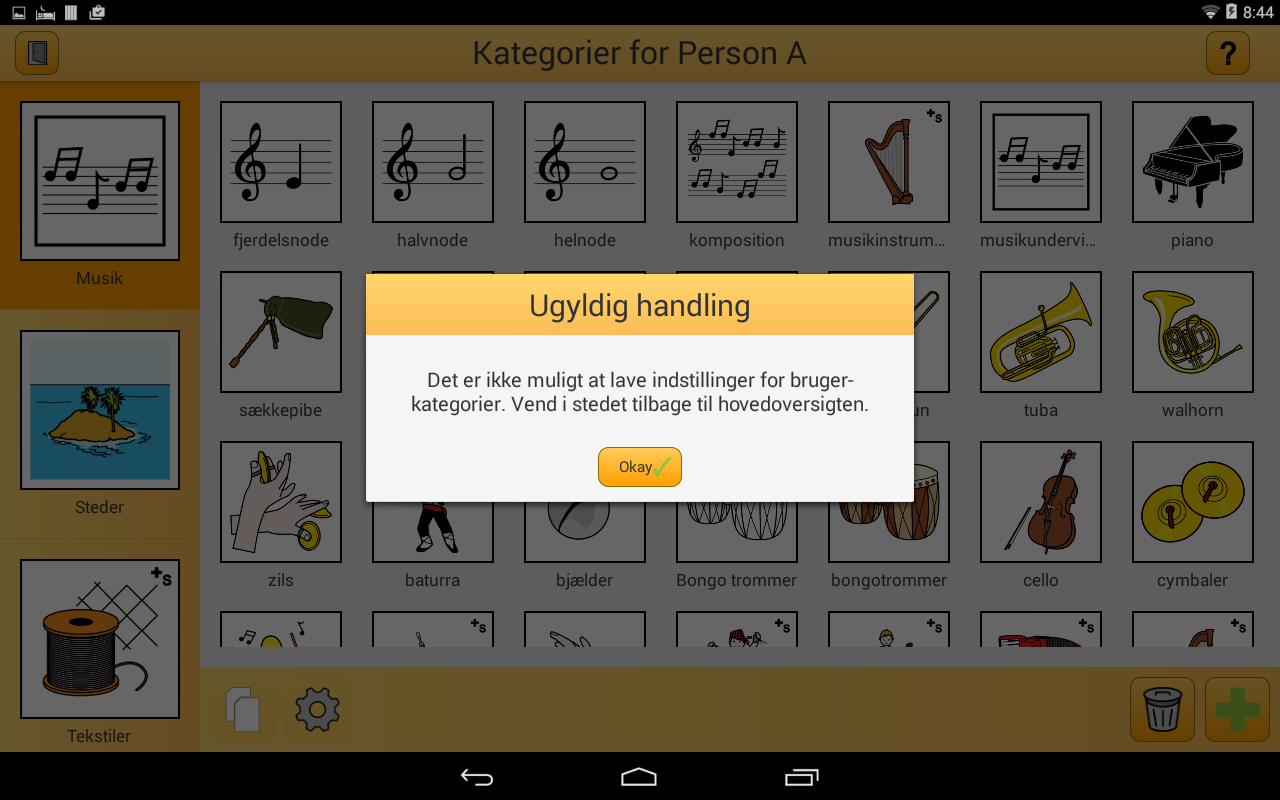
\includegraphics[width=0.75\textwidth]{sprint_three/locked_features_for_citizens/notifydialog_on_locked_click}
        \caption{Dialog shown when clicking disabled button}
        \label{fig:notifydialog_on_locked_click}
\end{figure}

%!TEX root = ../../../super_main.tex

\section{Memory Issues}
\label{sec:memory_issues}

The main purpose of the \ct is to manage and thereby display, add, and edit pictogram categories. We have to display series of pictograms in order to manage categories meaningfully. This caused some trouble because of the way the database components of the project are implemented. All database data abstraction classes that includes a bitmap, at the time of the third sprint, inherited from a class called \androidinline{BasicImageModel}. The problem with this class is that it lazy loads its bitmap and saves a reference to it until the \androidinline{BasicImageModel} itself is deallocated. The problem is then that we want to display potentially hundreds of pictograms, a few at a time, in a scrollable grid, i.e. an Android \androidinline{GridView}, on a device with a very limited amount of RAM. It may be that modern Android devices pack up to several gigabytes of RAM, but that does not mean that all of this RAM is available to all applications. In fact Android limits the heap size of each application to some device dependent limit as stated in the official Android application development memory guide \parencite{android_memory}. The guide text also recommends that applications only keep bitmaps in memory as long as they are currently shown on current screen of the graphical user interface. The memory limit forces us to only keep a very limited amount bitmaps in memory at any one time, compared to for instance a desktop environment where the virtual memory system will just page out bitmaps that were not used for some time. 

\subsection{Workaround}
\label{subsec:pictogram_workaround}

The database groups have been informed about the issue and we suggested a solution: Remove all references to the bitmaps kept by the \androidinline{BasicImageModel} and let the clients of the \androidinline{BasicImageModel} subclasses maintain the bitmap references. The database groups are working on a solution as of the end of sprint 3. \\

In order to make the \ct application work for the third Sprint Review Meeting, we implemented a workaround which allowed us to manage the references to bitmaps in the application code and not in the database abstraction code. \\

The workaround was implemented using Trail: The Reflection API in Java \parencite{java_trail_reflection}. What we did was make a deep copy of the \androidinline{BasicImageModel} object we want to display. We then load the bitmap, keeping a reference to it which we will manage ourself, from the deep copy of our object. The deep copy is then thrown away, insuring that we only have one reference to the bitmap.

\subsection{Android Adapters}

As described in \secref{sec:implementation_of_new_design} we use a combination of \androidinline{ListView} and \androidinline{Adapter} to display a list of items. \\

The Android framework provides a series of classes implementing an interface called \androidinline{Adapter} which makes it easy to map between collections of data and views. For instance when displaying a list of items in a \androidinline{ListView} which is a subclass of \androidinline{AdapterView}, or like in our case a scrolling grid of items in another subclass of \androidinline{AdapterView} called \androidinline{GridView}. A \androidinline{GridView} creates a scrollable grid of views, where the views are provided by its adapter. The \androidinline{AdapterView} subclasses all maintain a collection of views currently displayed plus some extras corresponding, in the case of the \androidinline{GridView}, to the next and previous row of views. \\

The views for the next row of data item is then generated by the adapter of the \androidinline{GridView} when the \androidinline{GridView} is scrolled to the next row of items by the user. The \androidinline{GridView} calls the \androidinline{Adapter} instance's \androidinline{getView} method once for each data item it wants to display each with the index, as an argument, of the desired data item. \\

The \androidinline{getView} method takes three arguments where one of them is called \androidinline{convertView} which is an instance of a previously discarded view corresponding to a data item that no longer needs to be displayed. This allows for reuse of the views so that the \androidinline{getView} does not need to create a new instance of a view every time it is called. Instead the \androidinline{getView} method implementation can simply reuse the \androidinline{convertView} \androidinline{View} instance and then load the relevant properties, for the data item at the calling index, in order to set them on the recycled view object. \\

All this together guarantees that there will only be up to some relatively small constant number of views, for the potentially large number of data items, in memory at any one time. If we let these views be the only objects keeping references to bitmaps, one reference per view, we would then be guaranteed to keep only a small constant number of bitmaps in memory at the same time assuming that the garbage collector can manage to free the memory fast enough when we load new bitmaps in and override the old bitmap references on the views. 

\subsection{View Element for Pictograms}
We packed our temporary solution, i.e our workaround from \secref{subsec:pictogram_workaround}, in a nice way to display pictograms called \androidinline{GirafPictogramItemView} see \secref{sec:consistent_pictograms}. One should in general no longer experience memory issues related to pictogram bitmaps as long as one uses \androidinline{GirafPictogramItemView} objects to display the pictograms managed by an Android \androidinline{Adapter} and as long as they do not attempt to display too many pictograms at once. \androidinline{GirafPictogramItemView} is a simple layout with an \androidinline{ImageView} at its core that lazy loads its bitmap on a background thread.


%!TEX root = ../../../super_main.tex

\chapter{Collaboration}

The following collaboration sections are the shared work of ours and another group. We sat down together and resolved shared, or similar, issues across the projects. The documented cases are far from the only collaborations we have participated in during the development of \giraf, but they are, however, the only collaborations that have been documented in detail. While collaborating with other groups, we used engineering practices like pair programming and code reviews. The collaborative work that we have conducted with these other groups is described in this chapter.

%!TEX root = ../../../super_main.tex
\section{Collaboration with Group SW606F15}
\label{sec:collaboration_with_group_sw606f15}

After a general GUI design meeting, a new sequence deletion method was suggested by the customers. Sequences are used in some of the applications that are being developed by the other GUI groups. Sequences are lists of pictograms that should be viewed in chronological order, when then represent a behavior/action sequence which the citizen can execute. This could for example be the order in which a citizen should dress, e.g. putting on his socks before shoes. \todo{Add a visual example of a sequence}. 
\\\\
The application \emph{Sequence} contains a set of different sequences. It is required of the application that different sequences may be removed. Previously when deleting sequences, the user would have to click a button to enter a ``Delete mode'' where, instead of clicking sequences to view them, clicks would delete the sequence. The customers requested the option to long-press a sequence to enter a ``Multi-selection mode'' where they were able to select multiple sequences in order to delete them. When a sequence is long pressed, the main menu is supposed to enter this mode and a trashcan button should appear in the top-bar. It should be possible to select and deselect sequences through regular press once inside the selection mode. It should furthermore be possible to deselect and exit the selection mode upon pressing the back button in the action bar.
\\\\
In our project, we had need for a feature just like this one, which instead of selecting sequences was focused around selecting pictograms inside categories. To quickly overcome this task, we grouped up with SW606f15, in order to resolve their issue first so we could implement the same structure in the two applications. The difference between the two projects is that our solution should only select a single item with a regular press, where theirs should be able to select multiple when initiated by a long-press.
\\\\
Previously, their project was based around the use of sequence objects and their respective ids to create views that represent the sequences. This resulted in not being able to find the view that belonged to the individual sequence, without passing both sequence and its view when using them in a method. This made it impossible to create the deselection feature when pressing the back button, since the back button was overriding the original \androidinline{onBackPressed} method, which does not take any parameters.
\\\\ 
Because of this we decided to implement a new data structure for their project which contains both a sequence and its respective view. This new structure made it possible to access the views that were selected and then deselect them when the back-button is pressed. 
\\\\
We furthermore implemented this using adapters as previously described, to improve performance when iterating through the list of sequences. This method of implementation could be directly transferred into our own project with minimal changes.

%!TEX root = ../../../super_main.tex

\section{Collaboration with Group SW613F15}
\label{sec:collaboration_with_group_sw613f15}

After the recent handover of \gc from group \emph{SW604F15} (us) to \emph{SW613F15}, it was discovered that a component in \ps (developed by \emph{SW613F15}) was not consistent with the design implemented in the \launcher (implemented by \emph{SW604F15}) regarding showing of multiple items, applications and pictograms respectively. This inconsistency can be seen in \figref{fig:collab_with_group_13}.

\begin{figure}[!htbp]
    \centering

    \begin{subfigure}[t]{0.75\textwidth}
        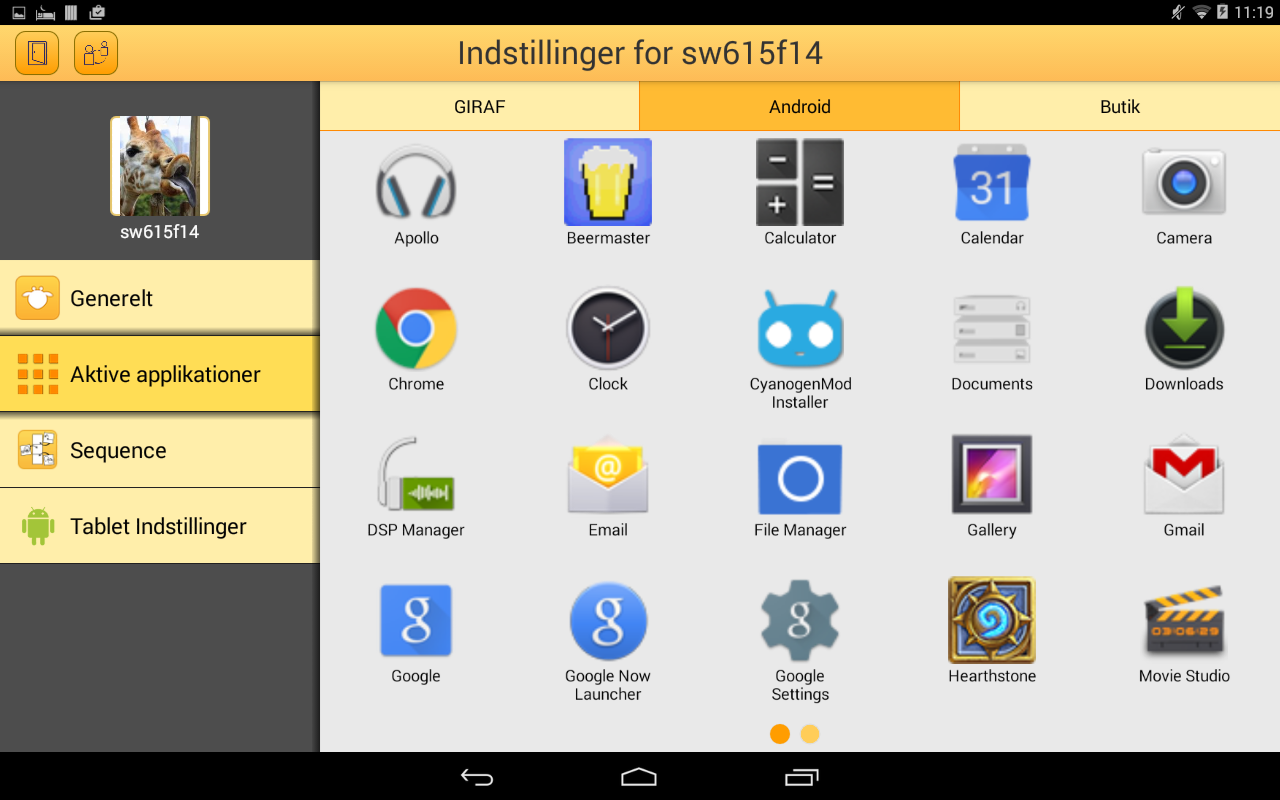
\includegraphics[width=\textwidth]{sprint_three/collab_with_group_13/launcher.png}
        \caption{The \launcher application}
        \label{fig:collab_with_group_13_launhcer}
        \vspace*{1cm}
    \end{subfigure}
    \hfill
    \begin{subfigure}[t]{0.75\textwidth}
        \includegraphics[width=\textwidth]{sprint_three/collab_with_group_13/pictosearch.png}
        \caption{The old \ps application}
        \label{fig:collab_with_group_13_pictosearch}
    \end{subfigure}
    
    \caption{Problem visualized}
    \label{fig:collab_with_group_13}
\end{figure}

Since \emph{SW604F15} had already spent some time on implementing a viewpager for this purpose, a solution for \ps was made in collaboration by these groups. A slight implementation difference was that the viewpager in the launcher is implementing using a \androidinline{FragmentAdapter}, whereas the viewpager in \ps is implemented using \androidinline{GridView}s. This soloution was though found to be inconsistent in regards to the other displays of pictograms and it was decided that there should be distinction between how applications should be presented and how pictograms and profile pictures should be presented. For this reasons we assisted \emph{SW613F15} to implemented a \androidinline{GridView} like the one implemented in \ct. The final result of \ps can be seen in \figref{fig:pictosearch}.


\begin{figure}[!htbp]
    \centering
    \includegraphics[width=0.75\textwidth]{sprint_three/pictosearch}
    \caption{Resulting application look for \ps}
    \label{fig:pictosearch}
\end{figure}